\chapter{Qiskit}
At the time of writing this we are using Qiskit 1.x to develop/ The following content has been copied directly from \href{https://docs.quantum.ibm.com/guides}{Qiskit IBM documentation}.
\section{Introduction to Qiskit}
The name "Qiskit" is a general term referring to a collection of software for executing programs on quantum computers. Most notable among these software tools is the \textbf{open-source Qiskit SDK}, and the \textbf{runtime environment} (accessed using Qiskit Runtime) through which you can execute workloads on IBM quantum computers. As quantum technology evolves, so does Qiskit, with new capabilities released every year that expands this core collection of quantum software.

In addition, many open-source projects are part of the broader Qiskit ecosystem. These software tools are not part of Qiskit itself, but rather interface with Qiskit and can provide valuable additional functionality. Parts of Qiskit environment are as shown in the figure \ref{fig:Qiskit}.

\begin{figure}
    \centering
    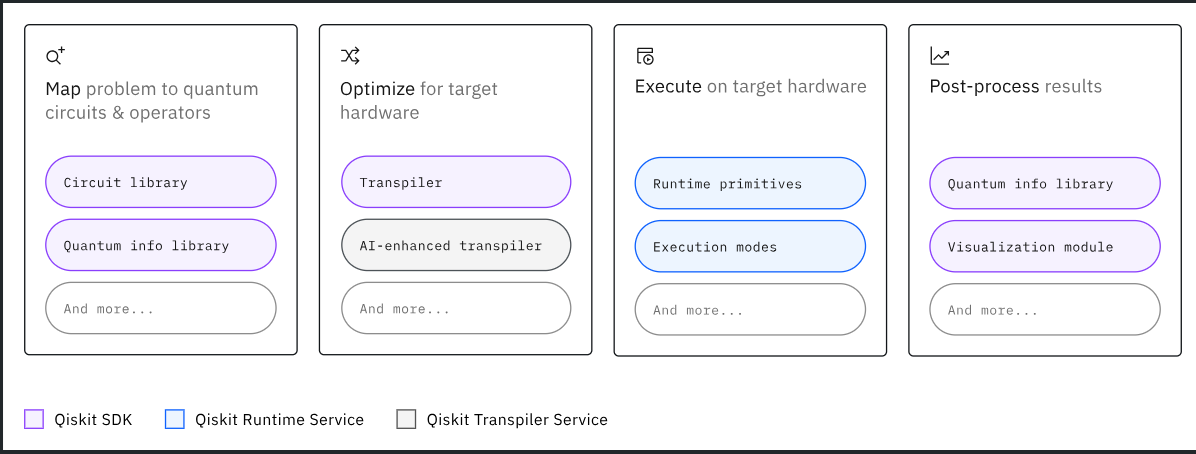
\includegraphics[width=1\linewidth]{Images/Qiskit.png}
    \caption{Qiskit Steps}
    \label{fig:Qiskit}
\end{figure}

\subsection{The Qiskit SDK}
The Qisit SDK (package name \href{https://pypi.org/project/qiskit/}{qiskit}) is an open-source SDK for working with quantum computers at the level of extended (static, dynamic, and scheduled) quantum circuits, operators and primitives. This library is the core component of Qiskit; it is the largest package under the Qiskit name with the broadest suit of tools for quantum computation, and many other components interface with it.
Some of the most useful features of the Qiskit SDK include:
\begin{itemize}
    \item Circuit-building tools (\href{https://docs.quantum.ibm.com/api/qiskit/circuit}{qiskit.circuit}) - For initializing and manipulating registers, circuits, instructions, gates, parameters, and control flow objects.
    \item Circuit library (\href{https://docs.quantum.ibm.com/api/qiskit/circuit_library}{qiskit.circuit.library}) - A vast range of circuits, instructions, and gates - key building blocks for circuit-based quantum computations.
    \item Quantum info library - (\href{https://docs.quantum.ibm.com/api/qiskit/quantum_info}{qiskit.quantum\_info}) - A toolkit for working with quantum states, operators and channels, using exact calculations (no sampling noise). Use this module to specify input observables and analyze fidelity of outputs from primitive queries.
    \item Transpiler (\href{https://docs.quantum.ibm.com/api/qiskit/transpiler}{qiskit.transpiler}) - For transforming and adapting quantum circuits to suit specific device topology, and optimizing for execution on real quantum systems.
    \item Primitives (\href{https://docs.quantum.ibm.com/api/qiskit/transpiler}{qiskit.primtives}) - The module that contains the base definitions and reference implementations of the \textbf{Sampler} and \textbf{Estimator} primitives, from which different quantum hardware providers can derive their own implementations. See more information about the Qiskit runtime primitives \href{https://docs.quantum.ibm.com/guides/primitives}{in the documentation}.
\end{itemize}
\subsection{Qiskit Runtime}
Qiskit Runtime is a cloud-based service for executing quantum computations on IBM Quantum hardware. The qiskit-ibm-runtime package is a client for that service,s an is the successor of the Qiskit IBM provider. The Qiskit Runtime service streamlines quantum computations and provides optimal implementation of the Qiskit primitives for IBM Quantum hardware. To get started with Qiskit runtime primitives, visit the \href{https://docs.quantum.ibm.com/guides/primitives}{documentation}.

With Qiskit Runtime you can choose to run your quantum programs on IBM Quantum hardware through the IBM Quantum Platform or IBM Cloud. See more information on selecting an IBM Quantum channel \href{https://docs.quantum.ibm.com/guides/setup-channel}{in the documentation}.

Qiskit Runtime is designed to use additional classical and quantum computer resources, including techniques such as error suppression and error mitigation, to return a higher-quality result from executing quantum circuits on quantum processors. Examples include dynamical decoupling for error suppression, and readout mitigation and zero-noise extrapolation (ZNE) for error mitigation. Learn how to configure these options on the \href{https://docs.quantum.ibm.com/guides/configure-error-mitigation}{Configure error mitigation} page.

Qiskit Runtime also includes three types of execution modes for running you quantum program on IBM hardware: Job, Session, and Batch, each of which have different use cases and implications for the quantum job queue. A Job is single query to a primitive that can be run over a specified number of shots. \href{https://docs.quantum.ibm.com/guides/sessions}{Sessions} allow you to efficiently run multiple jobs in iterative workloads on quantum computers. \href{https://docs.quantum.ibm.com/guides/run-jobs-batch}{Batch} mode allows you to submit all your jobs at once for parallel processing.

\subsubsection{Is Qiskit Runtime open-source?}
The short answer is, not all of it.  The Qiskit Runtime service software that handles the technicalities of running your quantum program on IBM Quantum device (including any error mitigation and suppression) is not open-source. However, the Qiskit Runtime client (the interface for users to access the Qiskit Runtime service), the Qiskit SDK running on the server side, and some of the software used for error mitigation, are open-source. To get involved with Qiskit open-source efforts, visit the GitHub organization at \href{https://github.com/Qiskit}{github.com/Qiskit} and \href{https://github.com/Qiskit-Extensions/}{github.com/Qiskit-Extensions}.

\subsection{Qiskit Serverless}
Creating utility-scale quantum applications generally requires a variety of computer resource requirements. Premium users can use Qiskit Serverless (package name qiskit-serverless) to easily submit quantum workflows for remote, managed execution. See more information \href{https://docs.quantum.ibm.com/guides/qiskit-serverless}{here} about how to use this collection of tools.

\subsection{Qiskit Transpiler as a Service}
The Qiskit transpiler service (package name \href{https://pypi.org/project/qiskit-transpiler-service/}{qiskit-transpiler service}) is a new experimental service that provides remote transpilation capabilities on the cloud to IBM Quantum Premium Plan users. In addition to the local Qiskit SDK transpiler capabilities, your transpilation tasks can benefit from both IBM Quantum cloud resources and AI-powered transpiler passes using this service. To learn more about how to integrate cloud-based transpilation into your Qiskit workflow you can \href{https://docs.quantum.ibm.com/guides/qiskit-transpiler-service}{check out the documentation}.

\subsection{The Qiskit ecosystem}
Beyond Qiskit there are many open-source projects that use the "Qiskit" name but are not part of Qiskit itself; rather, they interface with Qiskit and can provide valuable additional functionality to supplement the core Qiskit workflow. Some of these projects are maintained by IBM Quantum teams, whereas others are supported by the broader open-source community. The Qiskit SDK is designed in a modular, extensible way to make it easy for developers to create projects like these that extend its capabilities.
Some popular projects in the Qiskit ecosystem include:
\begin{itemize}
    \item Qiskit (qiskit-aer) - a package for quantum computing simulators with realistic noise models. It provides interfaces to run quantum circuits with or without noise using multiple different simulation methods. Maintained by IBM Quantum.
    \item qBraid SDK (qbraid) - a platform-agnostic quantum runtime framework for both quantum software and hardware providers, designed to streamline the full life cycle management of quantum jobs- from defining program specifications to job submission through to the post-processing and visualization of results. Maintained by qBraid.
    \item mthree (mthree) - a package for implementing M3(Matrix-free Measurement Mitigation), a measurement mitigation technique that solves for corrected measurement probabilities using a dimensionality reduction step followed by either direct LU factorization or a preconditioned iterative method that nominally converges $\mathcal{O}(1)$ steps, and can be computed in parallel. Maintained by IBM Quantum.
\end{itemize}
You can find a catalog of projects in the \href{https://qiskit.github.io/ecosystem/}{Qiskit ecosystem page}, as well as information about how to nominate your own project.

Please refer to the \href{https://www.youtube.com/watch?v=oaAjxcIFLtM}{YouTube lectures by Derek Wang}, research scientist at IBM for 
Coding with Qiskit 1.x. Qiskit version 1.x for utility scale for Quantum Computing. From installing Qiskit version1.x from scratch 
to learning how to run Quantum circuits both Unitary and dynamic based on some of the recent research papers by IBM Quantum. Using devices over 100 qubits using 
latest air suppression and mitigation techniques. Then learning how to contribute to the Qiskit ecosystem through open-source extra ordinate Abby Mitchell.

This is to get you up to speed with the latest developments on quantum computers for your own work. The foundation and focused on Qiskit 1 - an open source and freely available software development kit that allows you to program useful Quantum computational workflows. From designing Quantum Circuits and designing Quantum algorithms to submitting them to real Quantum Computers and orchestrating large scale complex workloads. Qiskit has now been for almost six years with previous iterations with Coding with Qiskit series. In the past few years with major developments in Quantum Computing most notably with the onset of the Utility era where Quantum Computers have now reached the level of scale and reliability such that researchers can now use them as legitimate tool for scientific exploration as highlighted by Research Nature paper by IBM Quantum. 

In utility era, the Quantum computational workflows will grow only in scale and complexity. There are high impact scientific papers that already use more than 100 qubits on IBM's 127 qubits chips, with thousands of gates in the circuit and tens and thousands of circuits in a workflow. With the proliferation of methods like circuit cutting and error mitigation that require fluid orchestration between multiple classical and quantum computers. The technology has evolved dramatically. Qiskit 1.0 is highly performant - faster and takes up less memory making it convenient for faster transpiler circuits with 100 plus qubits and thousands of gates. It is learner, removed meta package architecture, spun off packages like qiskit.algorithms into a separate one and deprecated modules like qiskit.opflow to make it more focused and maintainable. It is more stable. More features like Primitives in the form of sampler and estimator are now the access model for quantum hardware. Improved upon backend.run method from pre 1.0 versions. Primitives ensure that access to quantum hardware is consistent and reliable. Qiskit 1.0 is ready for dynamic circuits - enabling complex logic within a Quantum circuit more efficiently generating entangled states, teleport long range gates and path toward error correction. It is now easier to build on Qiskit. Like build your own transpiler plugin. extend qiskit capabilities for your own needs and share your code throughout the Qiskit ecosystem. 

\section{Install Qiskit}
Whether you will work locally or in a cloud environment, the first step for all users is to install Qiskit. For those wanting to run on a real system, your next step is to choose one of two channels in order to access IBM Quantum systems: IBM Quantum Platform or IBM Cloud.

Checkout the IBM Quantum Qiskit guide on \href{https://docs.quantum.ibm.com/guides/install-qiskit}{how to install} Qiskit and Qiskit Runtime and setup an \href{https://docs.quantum.ibm.com/guides/setup-channel}{IBM Quantum channel}.

\section{Anatomy of a Quantum Computing Service}
How does a Quantum program go from being on your laptop with you as the end user through to actually being run on a real quantum device?
\begin{figure}
    \centering
    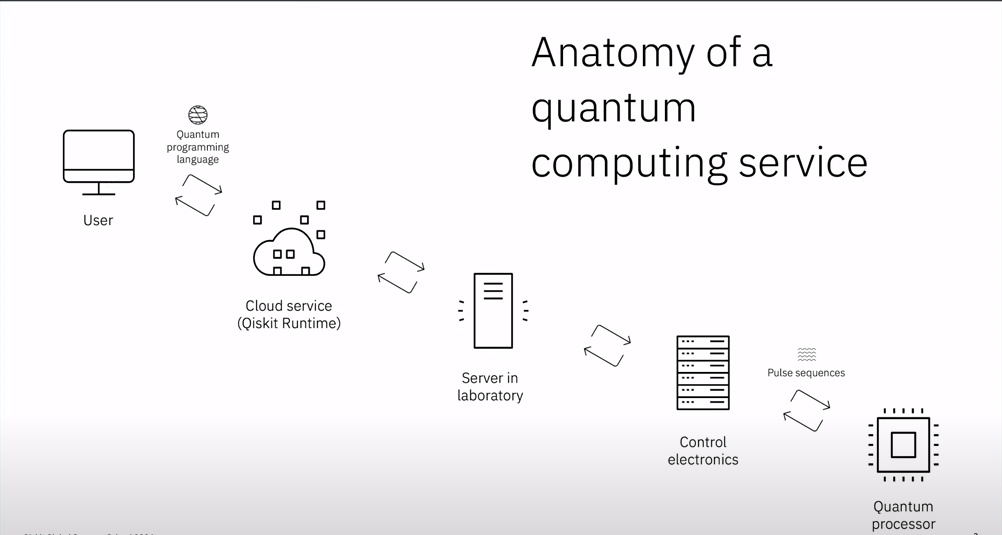
\includegraphics[width=0.75\linewidth]{Images/AnatomyofQC.png}
    \caption{Anatomy of Quantum Computing Service}
    \label{fig:AnatomyofQC}
\end{figure}
You need to use some Quantum programming language and in this case its going to be Qiskit to construct a quantum program. Then using a Cloud based service in this case called Qiskit Runtime to package up that program and send it through the cloud until it hits a server in a laboratory somewhere. Then the program will go through control electronics. The outcome of this will be your program will be converted to microwave pulse sequences that can then be run on real quantum processor. Once your program is run we will get the results back which will get propagated all the way back up the chain, back to you, the end user on your laptop. This gives you an overview at the high level view of the process and indicates the stuff going behind the scenes that maybe you as the end user aren't aware of. For the purpose of this lecture we are going to be focusing on user and Qiskit runtime (the parts with which user will be directly interacting with).

\begin{figure}
    \centering
    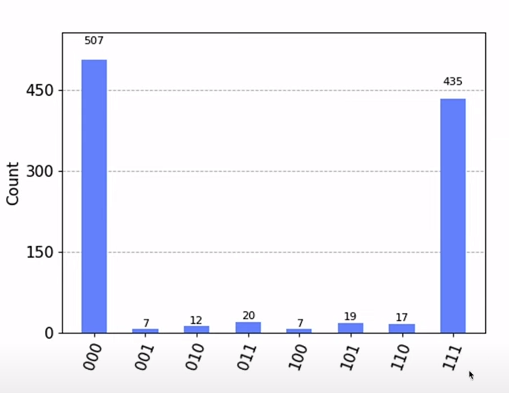
\includegraphics[width=0.75\linewidth]{Images/results_example.png}
    \caption{Example of final result}
    \label{fig:results_example}
\end{figure}
An example of final result is as shown in the figure \ref{fig:results_example}. You will get a series of bit strings many zeros and ones, these in a classical format. you will typically have run the program many times on the quantum device and so you will get probabilities back on how did you get a certain bit string more so than others. Thus as can be seen through the graph that the quantum program gave a lot of results that were 000 and 111 which is probably the answer to the program that you are trying to run. We also get a lot of much smaller counts of different bit strings here. And this, shows that there are some errors on the quantum device. Quantum devices are not perfect. You will often get small numbers of incorrect bit strings from the outcome of your experiment. This is why you have to run your program multiple times so that you can start to see these are where the errors are. We can also talk about ways to prevent or mitigate these kinds of errors. Ideally we would only want to see two bars in the image.

\textbf{What is Qiskit?}\\
\begin{itemize}
\item Qiskit SDK is an open-source SDK for working with Quantum Computers at the level of extended quantum circuits, operators and primitives. You can find the code and documentation here. Currently version 1.0 is used released on Feb 2024.

\item Qiskit runtime is a cloud based service for executing quantum computations on IBM Quantum hardware. Qiskit runtime services is not open-source but the client that you use to interact with that service is. And you can check that repository on GitHub along with the documentation. Currently version 2 is used (released March 2024).

\item Qiskit patterns is a framework for breaking down domain-specific problem into stages to build a quantum program. It is guidelines on how to construct a full quantum program including everything from building your initial circuit through to running it on real hardware and getting the results at the end.

\item The Qiskit Ecosystem is a collection of software and projects that build or extend Qiskit. These are additional packages which are building on Qiskit which can be an addition to your toolbox of Qiskit SDK and Qiskit runtime. These are referred to as part of the Qiskit ecosystem. It can be found here to find the catalog some maintained by IBM and some maintained by members of the open source community.
\end{itemize}

\subsection{Getting set up with Qiskit}
\begin{lstlisting}
pip install 'qiskit[visualization]' # Install Qiskit SDK with the additional visualization capabilities
pip install qiskit-ibm-runtime
\end{lstlisting}

For visualizing circuits and results install Qiskit with visualization add-on.

To access IBM hardware, set up your credientials through one of:
\begin{itemize}
    \item IBM Quantum Platform
    \item IBM cloud
\end{itemize}

\subsection{Qiskit Patterns}

\section{Qiskit 101}
Qiskit 101 is exactly what it sounds like: a first introduction to Qiskit. There are no prerequisite for this course, though partners with some coding experience and who have played a bit with Qiskit will benefit the most. The course is focused on starting with IBM Quantum, building your fist quantum circuits, and testing the results by running code on simulators. Topics covered include quantum circuits, quantum gates, and Qiskit Runtime Primitives. Qiskit 101 is geared primarily toward future technical practioners of quantum computing.

\subsection{Qiskit 101 traning session}
Recoding of the latest live session from June 11, 2024. Estimator(mode=backend)

\section{Explore gates and circuits with IBM Quantum Composer}
\textbf{What is it?}\\
IBM Quantum Composer is a graphical quantum programming tool that lets you drag and drop operations to build quantum circuits and run them on real quantum hardware or simulators.

\textbf{What can it do?}\\
\begin{itemize}
    \item \textbf{Visualize qubit states:} See how changes to your circuit affect the state of qubits, shown as an interactive q-shpere, or histogram showing measurement probabilities or statevector simulations.
    \item \textbf{Run on quantum hardware:} Run your circuits on real quantum hardware to understand the effects of device noise.
    \item \textbf{Automatically generate code:} Instead of writing code by hand, automatically generate OpenQASM or Python code that behaves the same way as the circuit you created with Quantum Composer.
\end{itemize}

\textbf{Tour of the interface}\\
IBM Quantum Composer has a customizable set of tools that allow you to build, visualize and run quantum circuits on quantum systems of simulators. Use the more options menu on each window to access additional tools and actions.
\begin{enumerate}
    \item \textbf{Tools panels:} Use the side panel to view your files or jobs, or the documentation. To close the side panel, click the icon for the open tab.
    \item \textbf{Menu bar:} use these menus to create a new circuit, manage saved circuits and registers, customize your workspace, and more.
    \item \textbf{Run area:} Change the run settings and then run your circuit on a quantum system or simulator.
    \item \textbf{Composer files:} The circuits you create save automatically and display in the composer files panel.
    \item \textbf{Circuit name:} - Click here to name your circuit.
    \item \textbf{Operations catalog:} These are the building blocks of quantum circuits. Drag and drop these gates and other operations onto the graphical circuit editor. Different types of gates are grouped together by color. For example, classical gates are dark blue, phase gates are light blue, and non-unitary operations are grey.
    \item \textbf{Code editor:} Use the View menu to open or close the code editor, which allows you to view and edit the OpenQASM or Qiskit code for the circuit.
    \item \textbf{Graphical circuit editor:} This is where you build a circuit. Drag gates and other operations onto the horizontal qubit ``wires" that make up your quantum register. To remove a gate from a wire, select the gate and click the trash icon. To edit the parameters and settings on gates that support editing, select the gate on the graphical editor and click edit.
    \item \textbf{Toolbar:} Access frequently used tools to undo and redo actions, change the gate alignment, and switch to inspec mode. Inspect mode lets you view a step-by-step view of the qubit states as your circtui computation evolves. 
\end{enumerate}




\chapterreferences
